%%%%%%%%%%%%%%%%%%%%%%%%%%%%%%%%%%%%%%%%%%%%%%%%%%%%%%%%%%%%%%%%%%%%%%
% LaTeX Template: Beamer arrows
%
% Source: http://www.texample.net/
% Feel free to distribute this template, but please keep the
% referal to TeXample.net.
% Date: Nov 2006
% 
%%%%%%%%%%%%%%%%%%%%%%%%%%%%%%%%%%%%%%%%%%%%%%%%%%%%%%%%%%%%%%%%%%%%%%
% How to use writeLaTeX: 
%
% You edit the source code here on the left, and the preview on the
% right shows you the result within a few seconds.
%
% Bookmark this page and share the URL with your co-authors. They can
% edit at the same time!
%
% You can upload figures, bibliographies, custom classes and
% styles using the files menu.
%
% If you're new to LaTeX, the wikibook is a great place to start:
% http://en.wikibooks.org/wiki/LaTeX
%
%%%%%%%%%%%%%%%%%%%%%%%%%%%%%%%%%%%%%%%%%%%%%%%%%%%%%%%%%%%%%%%%%%%%%%

\documentclass[usenames,dvipsnames]{beamer} %
\usetheme{Madrid}
\usecolortheme{beaver}
\usepackage[latin1]{inputenc}
\usefonttheme{professionalfonts}
\usepackage{pifont}
\usepackage{tikz}
\usepackage{amsmath,amsfonts,amssymb}
\usepackage{verbatim}
\usepackage{hyperref}
\usepackage{subfigure}
\usepackage{bm}
\usepackage{gensymb}
\usepackage{bbm}

\usepackage{xcolor}
\usepackage{media9}
\usepackage{animate}
\usepackage{booktabs}
\usepackage{color}
\usepackage{listings}

\definecolor{deepblue}{rgb}{0,0,0.5}
\definecolor{deepred}{rgb}{0.6,0,0}
\definecolor{deepgreen}{rgb}{0,0.5,0}

\DeclareMathOperator*{\argmax}{arg\,max}
\DeclareMathOperator*{\argmin}{arg\,min}

\usetikzlibrary{arrows,shapes}

%\beamerdefaultoverlayspecification{<+->}

\setbeamercolor{itemize item}{fg=red}
\setbeamercolor{itemize subitem}{fg=BrickRed}
\setbeamercolor{itemize subsubitem}{fg=black}

\setbeamertemplate{itemize item}[square]
\setbeamertemplate{itemize subitem}[circle]
\setbeamertemplate{itemize subsubitem}[triangle]

\setbeamertemplate{caption}[numbered]

\newcommand\bred[1]{\textcolor{red}{\textit{#1}}}
\newcommand\bblue[1]{\textcolor{blue}{\textit{#1}}}

\newcommand\vari[1]{\textcolor{BrickRed}{\texttt{#1}}}
\newcommand\defi[1]{\textcolor{NavyBlue}{\textit{#1}}}

\renewcommand{\figurename}{Figura}
\newcommand{\matr}[1]{\mathbf{#1}}

\author{MSc. Diego Porres}
\title{Elements of Machine Learning}
\subtitle{Clasificaci\'on}
\institute[UFM]{
\includegraphics[height=0.73cm, width=3.3cm]{images/LogotipoUFM_interna.png}}
\date{Febrero 2019}


\begin{document}

\frame{\titlepage}

\begin{comment}
:Title: Beamer arrows
:Tags: Remember picture, Beamer, Physics & chemistry, Overlays
:Use page: 3

With PGF/TikZ version 1.09 and later, it is possible to draw paths between nodes across
different pictures. This is a useful feature for presentations with the
Beamer package. In this example I've combined the new PGF/TikZ's overlay feature
with Beamer overlays. Download the PDF version to see the result.

**Note.** This only works with PDFTeX, and you have to run PDFTeX twice.

| Author: Kjell Magne Fauske

\end{comment}


% For every picture that defines or uses external nodes, you'll have to
% apply the 'remember picture' style. To avoid some typing, we'll apply
% the style to all pictures.
\tikzstyle{every picture}+=[remember picture]

% By default all math in TikZ nodes are set in inline mode. Change this to
% displaystyle so that we don't get small fractions.
\everymath{\displaystyle}

\begin{frame}
\begin{center}
	\item Some of the figures in this presentation are taken from \textit{An Introduction to Statistical Learning, with applications in R}  (Springer, 2013) with permission from the authors: G. James, D. Witten, T. Hastie and R. Tibshirani
	\item
	\item Some of the figures in this presentation are taken from \textit{The Elements of Statistical Learning}  (Springer, 2009) with permission from the authors: T. Hastie, R. Tibshirani, and J. Friedman
\end{center}
\end{frame}

\begin{frame}\frametitle{Intro (1)}
    \begin{itemize}
    	\item Pasamos ahora al caso en donde la respuesta $Y$ es cualitativa, por lo que la denotaremos por $G$.
    	\item A las variables cualitativas tambi\'en se les llama \defi{categ\'oricas}.
    	\item \textbf{Objetivo:} \defi{clasificar} a la observaci\'on $X$ en una de las $K$ distintas categor\'ias (no ordenadas).
    	\item $G$ tomar\'a valores en un conjunto finito $\mathcal{G}$, por lo que:
    	\[ G:\mathbb{R}^p\rightarrow \mathcal{G}=\{1,\dotsc, K\} \]
        \begin{itemize}
        	\item En general estamos m\'as interesados en calcular las probabilidades que $X$ pertenezca a cada clase.
        \end{itemize}
    \end{itemize}
\end{frame}

\begin{frame}{Intro (2)}
	\begin{itemize}
		\item A las t\'ecnicas usadas para clasificar datos se les conoce como \defi{clasificadores}.
		\item Analizaremos a	 los siguientes clasificadores:
		\begin{itemize}
			\item Regresi\'on log\'istica
			\item An\'alisis discriminante lineal (LDA)
			\item K-vecinos cercanos (KNN)
		\end{itemize}
		\item Veremos otros clasificadores m\'as adelante. 
	\end{itemize}
\end{frame}

\begin{frame}{Intro (3)}
	\begin{itemize}
		\item Los problemas de clasificaci\'on son m\'as comunes que los de regresi\'on.
		\item Algunos ejemplos son:
		\begin{itemize}
			\item Si una persona ingresa a la sala de emergencia de un hospital con un conjunto de s\'intomas debido a uno de tres posibles enfermedades, ?`qu\'e enfermedad es la que padece?
			\item El servicio de banca en l\'inea de un banco determina si una transacci\'on es o no  fraudulenta, tomando a la direcci\'on IP, historial de transacciones, hora de la transacci\'on, etc.
			\item Clasificar a un correo como normal o \textit{spam}, bas\'andonos en las palabras en el cuerpo del correo y del t\'itulo, etc.
			\item Predecir si un individuo va a incurrir en un \vari{impago} (\vari{default}) en su tarjeta de cr\'edito, dado su salario anual, balance mensual en su tarjeta de cr\'edito, etc.
		\end{itemize}
	\end{itemize}
\end{frame}

\begin{frame}\frametitle{Datos de \href{https://github.com/JWarmenhoven/ISLR-python/blob/master/Notebooks/Data/Default.xlsx}{\vari{Default}}}
    \begin{figure}
    \centering
        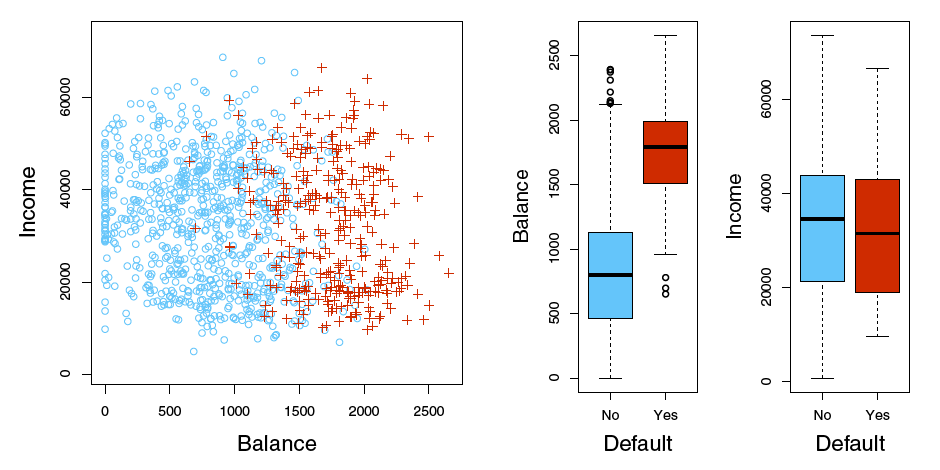
\includegraphics[width=0.70\textwidth]{images/islr/fig_4_1.png}
    \caption{Graficamos los datos de \href{https://github.com/JWarmenhoven/ISLR-python/blob/master/Notebooks/Data/Default.xlsx}{\vari{Default}} (datos simulados). A la izquierda, vemos la relaci\'on entre el balance en la tarjeta de cr\'edito vs. el ingreso anual (en \$). Los individuos que incurrieron en un impago se muestran en \textcolor{BrickRed}{rojo}, mientras los que no se muestran en \textcolor{Cerulean}{azul}. A la derecha, tenemos diagramas de cajas del balance e ingresos en funci\'on del estado de impago. (La divisi\'on de los datos casi nunca es as\'i de clara en la vida real.)}
    \label{fig:islr_4-1}
    \end{figure}
\end{frame}

\begin{frame}\frametitle{Intro (4)}
\begin{itemize}
	\item $G$ dividir\'a a nuestro espacio en regiones etiquetadas de acorde a su clasificaci\'on. 
	\item Las fronteras entre estas regiones se les llama \defi{fronteras de decisi\'on}.
	\item Cuando las fronteras son lineales, denominamos al clasificador como \defi{lineal}.
	\item Podemos expandir a nuestro conjunto de variables $X_1,\dotsc,X_p$ a que incluya tambi\'en los productos y cuadrados: $X_1^2,\dotsc, X_p^2, X_1 X_2, X_1 X_3, \dotsc$.
	\item \'Esto nos agregar\'a $\binom{p}{2}=p(p+1)/2$ variables.
	\item Fronteras de decisi\'on lineales en este espacio aumentado corresponder\'an a fronteras de decisi\'on \defi{cuadr\'aticas} en el espacio original.
\end{itemize}
\end{frame}

\begin{frame}\frametitle{Fronteras de Decisi\'on}
\begin{figure}
	\centering
	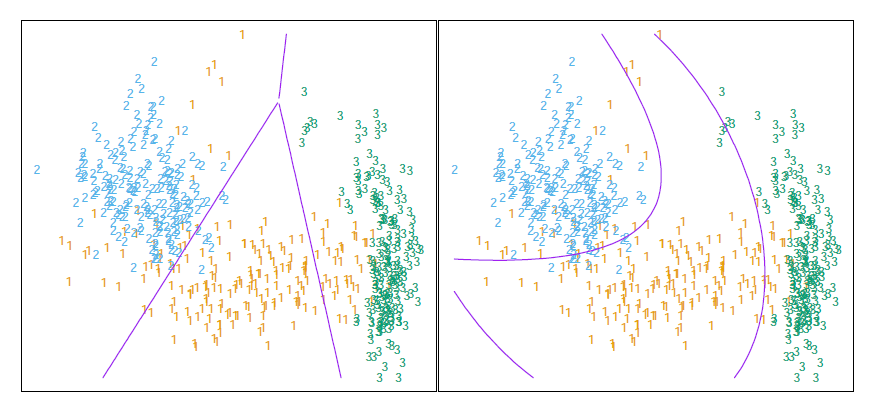
\includegraphics[width=0.70\textwidth]{images/esl/fig_4_1.png}
	\caption{A la izquierda graficamos los datos de tres clases con fronteras de decisi\'on lineales. A la derecha graficamos las fronteras de decisi\'on cuadr\'aticas. \'Estas fueron obtenidas al encontrar las fronteras de decisi\'on lineales en el espacio pentadimensional $X_1,X_2,X_1 X_2, X_1^2, X_2^2$. L\'ineas en dicho espacio son curvas cuadr\'aticas en el espacio original.}
	\label{fig:esl_4-1}
\end{figure}
\end{frame}


\begin{frame}\frametitle{?`Cu\'ando aparece una frontera de decisi\'on lineal?}
	\begin{itemize}
		\item Nuestro objetivo, entonces, es de aprender una \defi{funci\'on discriminante} $\delta_k (x)$ para cada clase $k$ y establecer:
		\begin{equation}\label{eq:esl_4-discr} 
		G(x) = \argmax_k \delta_k (x)
		\end{equation}
		\item $G$ generar\'a una frontera de decisi\'on lineal si existe alguna transformaci\'on mon\'otona $g$ de $\delta_k (x)$ que sea lineal.
		\item Es decir, $g$ es una funci\'on mon\'otona tal que
		\[ g(\delta_k (x)) = \gamma_{k0} + \gamma_{k}^{\top}x \]
	\end{itemize}
\end{frame}

\begin{frame}\frametitle{Un ejemplo de una frontera de decisi\'on lineal}
	\begin{itemize}
		\item Por ejemplo, podemos usar a las probabilidades a posteriori $\mathbb{P}[G=k|X=x]$ como nuestras funciones discriminantes para dos clases:
		\begin{equation}\label{eq:esl_4-1}
		\begin{aligned}
		\delta_1 (x)=\mathbb{P}[G=1|X=x]&=\frac{\exp{(\beta_0 + \beta^\top x)}}{1+\exp{(\beta_0 + \beta^\top x)}}\\
		\delta_2 (x)=\mathbb{P}[G=2|X=x]&=\frac{1}{1+\exp{(\beta_0 + \beta^\top x)}}
		\end{aligned}
		\end{equation}
		\item Podemos aplicar a la transformaci\'on mon\'otona (\defi{logit}) $g(p)=\log{(p/(1-p))}$ y vemos que:
		\begin{equation}\label{eq:esl_4-2}
		\log{\frac{\mathbb{P}[G=1|X=x]}{\mathbb{P}[G=2|X=x]}} = \beta_0 + \beta^\top x
		\end{equation}
	\end{itemize}
\end{frame}

\begin{frame}\frametitle{?`Por qu\'e no usamos regresi\'on lineal? (1)}
\begin{itemize}
	\item Para una respuesta \defi{binaria} (de dos niveles) como en el caso de los datos de \vari{Default} tendremos:
	\begin{equation*}
G = \begin{cases}
0 & \text{ si la persona \vari{No} incurri\'o en un impago}\\
1 & \text{ si la persona \vari{Si} incurri\'o en un impago}
\end{cases}
	\end{equation*}
	\item ?`Qu\'e pasa si realizamos una regresi\'on lineal de $G$ sobre $X$ y lo clasificamos como \vari{Si} si $\hat{G}>0.5$?
	\item En este caso, la regresi\'on lineal realizar\'a un buen trabajo y ser\'a equivalente al \defi{an\'alisis discriminante lineal (LDA)}.
	\begin{itemize}
		\item El $X \hat \beta$ obtenido ser\'a un estimador de $\mathbb{P}[\vari{Si}|X]$.
		\item Sin embargo, algunas de nuestras estimaciones estar\'an fuera del intervalo $[0,1]$.
		\item Para \'esta tarea, la \defi{regresi\'on log\'istica} es m\'as adecuada.
	\end{itemize}
\end{itemize}
\end{frame}

\begin{frame}\frametitle{Fronteras de Decisi\'on}
\begin{figure}
	\centering
	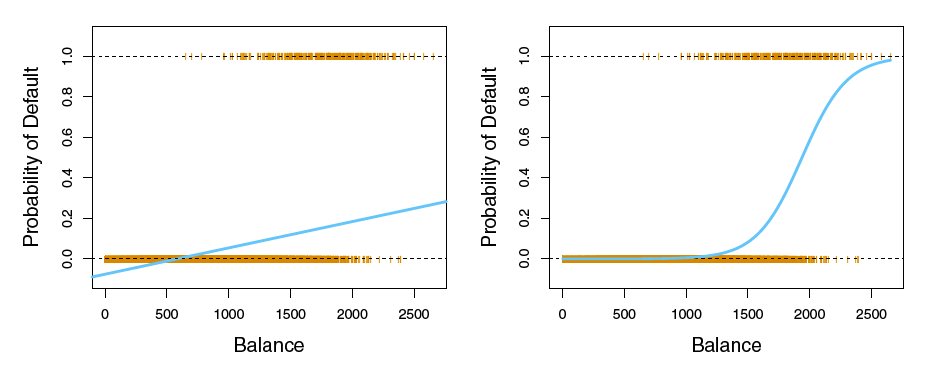
\includegraphics[width=0.8\textwidth]{images/islr/fig_4_2.png}
	\caption{Clasificando a los datos de \vari{Default} en funci\'on del \vari{Balance}. A la izquierda, estimamos las probabilidades usando regresi\'on lineal. N\'otee que algunas de las probabilidades son \textit{negativas}, mientras que en los datos de \vari{Balance} m\'aximo, la probabilidad llega como m\'aximo al 30\%. A la derecha, predecimos la probabilidad de \vari{impago} usando regresi\'on log\'istica. Los datos se presentan de color \textcolor{orange}{naranja} e indican la verdadera clasificaci\'on de los mismos.}
	\label{fig:islr_4-2}
\end{figure}
\end{frame}

\begin{frame}\frametitle{?`Por qu\'e no usamos regresi\'on lineal? (2)}
\begin{itemize}
	\item Suponga ahora que tratamos de clasificar, dados los s\'intomas $X_1,\dotsc,X_p$, la condici\'on/enfermedad que sufre un paciente:
	\begin{equation*}
	G = \begin{cases}
	1 & \text{ si es un \vari{infarto}}\\
	2 & \text{ si es una \vari{sobredosis}}\\
	3 & \text{ si es un \vari{ataque epil\'eptico}}
	\end{cases}
	\end{equation*}
	\item El s\'olo hecho de haber ordenado a las clases implica que la diferencia entre \'estas es la misma.
	\item El \'orden utilizado es arbitrario y, de haber usado otro, la regresi\'on lineal predecir\'ia distintos valores en $\mathcal{T}_{\text{Te}}$.
	\item Por lo tanto, \defi{Regresi\'on log\'istica multinomial} o \defi{An\'alisis discriminante} son m\'as apropiados.
\end{itemize}
\end{frame}

\begin{frame}\frametitle{Fronteras de decisi\'on parar tres clases}
\begin{figure}
	\centering
	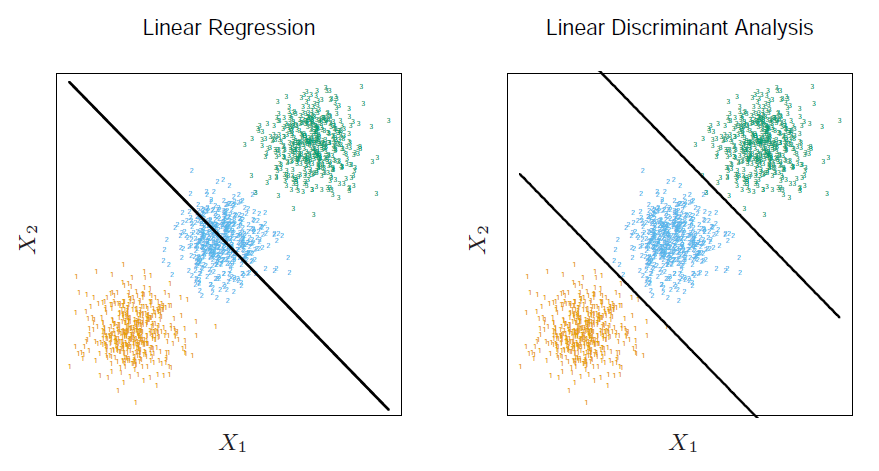
\includegraphics[width=0.8\textwidth]{images/esl/fig_4_2.png}
	\caption{Para datos de tres clases en $\mathbb{R}^2$, a la izquierda vemos que las fronteras de decisi\'on generadas por una regresi\'on lineal \textit{enmascaran} a la clase de enmedio (nunca domina). En cambio, a la derecha vemos las fronteras generadas por el an\'alisis discriminante lineal, el cual separa f\'acilmente a las clases.}
	\label{fig:esl_4-2}
\end{figure}
\end{frame}

\begin{frame}\frametitle{Enmascaramiento de los datos}
\begin{figure}
	\centering
	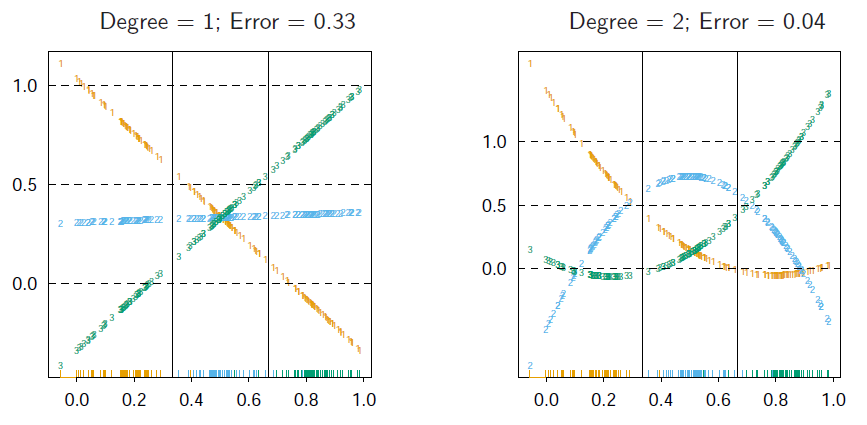
\includegraphics[width=0.8\textwidth]{images/esl/fig_4_3.png}
	\caption{Realizamos \textit{rug plots} para cada clase, y graficamos la probabilidad estimada por la regresi\'on lineal. A la izquierda, vemos que la clase 2 est\'a siempre enmascarada por las otras dos clases. A la derecha, realizamos la regresi\'on lineal con polinomios cuadr\'aticos, lo cual decrece el error de manera considerable. El error de Bayes es de $0.025$ y es el realizado por el an\'alisis discriminante lineal.}
	\label{fig:esl_4-3}
\end{figure}
\end{frame}

\begin{frame}\frametitle{Regresi\'on Log\'istica}
\begin{itemize}
	\item Consideramos de nuevo a los datos de \vari{Default} cuyas clases definimos como \vari{Si} o \vari{No}.
	\item No queremos conseguir a $G$ directamente, sino a la probabilidad de que pertenezca a cualquiera de las dos clases, e.g.:
	\[ p(\vari{Balance})=\mathbb{P}[\vari{Impago}=\vari{Si}|\vari{Balance}] \]
	\item Predecimos que $\vari{Impago}=\vari{Si}$ para toda persona que cumpla con $p(\vari{Balance})>\alpha$, donde $\alpha$ es un \defi{umbral} previamente establecido.
	\begin{itemize}
		\item Para algunas aplicaciones basta $\alpha=0.5$, pero con otras m\'as conservativas, quiz\'a sea mejor $\alpha=0.1$.
	\end{itemize} 
\end{itemize}
\end{frame}

\begin{frame}\frametitle{El modelo log\'istico}
\begin{itemize}
	\item Abreviemos la relaci\'on de manera $p(X)=\mathbb{P}[G=1|X]$. ?`C\'omo podemos modelar \'esta relaci\'on?
	\item Si usamos un modelo lineal, obtendremos los resultados de la Figura \ref{fig:islr_4-2}, con algunas probabilidades siendo menores a 0.
	\item Para evitar \'esto, usaremos a la \defi{funci\'on log\'istica}:
	\begin{equation}\label{eq:islr_4-2}
	p(X)=\frac{\rm{e}^{\beta_0 + \beta_1 X}}{1+\rm{e}^{\beta_0 + \beta_1 X}}=\frac{1}{1+\rm{e}^{-\beta_0 - \beta_1 X}}=\sigma(\beta_0+\beta_1 X)
	\end{equation}
	\begin{itemize}
		\item $\sigma$ es la \defi{funci\'on sigmoide}
	\item $\lim_{X\rightarrow+\infty}p(X)=1$,  $\lim_{X\rightarrow-\infty}p(X)=0$
	\end{itemize}
	\item A $p(X)/(1-p(X))$ se les llama las \defi{posibilidades (odds)}.
	\item El \defi{logit/log-odds} o \defi{posibilidad logar\'itmica} se define como:
	\begin{equation}\label{eq:islr_4-4}
	\log{\left( \frac{p(X)}{1-p(X)} \right)}=\beta_0 + \beta_1 X
	\end{equation}
\end{itemize}
\end{frame}

\begin{frame}\frametitle{Estimando los coeficientes de regresi\'on}
\begin{itemize}
	\item Podr\'iamos utilizar m\'inimos cuadrados para encontrar a los par\'ametros \'optimos de \ref{eq:islr_4-4}, pero preferimos utilizar el m\'etodo de \defi{m\'axima verosimilitud}.
	\item Queremos encontrar a $\hat \beta_0$ y $\hat \beta_1$ tales que $p(X)$ est\'e lo m\'as cercano posible a 1 para los individuos que incurran en impago y a 0 para aquellos que no.
	\item Podemos formalizar a \'esto mediante la \defi{funci\'on de verosimilitud}:
	\begin{equation}\label{eq:islr_4-5}
	\ell(\beta_0, \beta_1)=\prod_{i:y_i=1}p(x_i)\prod_{i':y_{i'}=0}(1-p(x_{i'}))
	\end{equation}
	\item Por lo tanto:
	\begin{equation}\label{eq:islr_4-5a}
	\hat \beta_0, \hat \beta_1 = \argmax_{\beta_0, \beta_1} \ell (\beta_0, \beta_1)
	\end{equation}
\end{itemize}
\end{frame}

\begin{frame}\frametitle{Funci\'on de m\'axima verosimilitud}
\begin{itemize}
	\item La \defi{verosimilitud} nos da la probabilidad de los ceros y unos observados en los datos.
	\item Por ende, queremos maximizar a $\ell (\beta_0, \beta_1)$.
	\item Si $\hat \beta_1>0$, entonces un incremento en el \vari{balance} est\'a asociado con un incremento en la probabilidad de incurrir en un \vari{impago}.
	\item $\hat \beta_0$ no nos ser\'a de interes en particular; s\'olo nos servir\'a a la hora de ajustar las probabilidades a ser las proporciones de unos en los datos.
	\item La \defi{verosimilitud logar\'itmica} se define como:
	\begin{align*} \log{\ell(\beta_0, \beta_1)}&= \log{\left( \prod_{i:y_i=1}p(x_i)\prod_{i':y_{i'}=0}(1-p(x_{i'}))\right)}\\
	&=\sum_{i:y_i=1}\log{p(x_i)} + \sum_{i':y_{i'}=0}\log{(1-p(x_{i'}))}\\
	&=\sum_{i=1}^n \left\{ y_i \log{p(x_i)} + (1-y_i)\log{(1-p(x_{i}))} \right\}
	\end{align*}
\end{itemize}
\end{frame}

\begin{frame}[fragile]\frametitle{C\'odigo coeficientes de regresi\'on log\'istica (1)}
\begin{semiverbatim}
	\small{\textcolor{deepblue}{import} pandas \textcolor{deepblue}{as} pd
	\textcolor{deepblue}{import} statsmodels.api \textcolor{deepblue}{as} sm
	\textcolor{deepblue}{import} statsmodels.formula.api \textcolor{deepblue}{as} smf
	
	df = \href{https://pandas.pydata.org/pandas-docs/stable/reference/api/pandas.read_excel.html}{pd.read\_excel}(\href{https://goo.gl/qSE6q8}{"https://goo.gl/qSE6q8"})
	
	# .factorize() nos regresa dos objetos: un array con etiquetas
	# y uno con valores unicos. Solo nos interesa el primero:
	df["default2"] = df.default.\href{https://pandas.pydata.org/pandas-docs/version/0.23.4/generated/pandas.factorize.html}{factorize()}[0]
	
	y = df.default2
	X = \href{http://www.statsmodels.org/devel/generated/statsmodels.tools.tools.add_constant}{sm.add\_constant}(df.balance)
	
	est = smf.\href{https://www.statsmodels.org/dev/generated/statsmodels.discrete.discrete_model.Logit.html}{Logit}(\href{https://docs.scipy.org/doc/numpy-1.15.0/reference/generated/numpy.ravel.html}{y.ravel()}, X).fit()
	
	>>> print(est.summary().tables[1])
}
\end{semiverbatim}
\end{frame}

\begin{frame}[fragile]\frametitle{C\'odigo coeficientes de regresi\'on log\'istica (2)}
\begin{semiverbatim}
	\small{\textcolor{deepblue}{import} pandas \textcolor{deepblue}{as} pd
		\href{https://scikit-learn.org/stable/modules/classes.html#module-sklearn.linear_model}{\textcolor{deepblue}{import} sklearn.linear\_model \textcolor{deepblue}{as} skl\_lm}
		
		df = \href{https://pandas.pydata.org/pandas-docs/stable/reference/api/pandas.read_excel.html}{pd.read\_excel}(\href{https://goo.gl/qSE6q8}{"https://goo.gl/qSE6q8"})
		
		df["default2"] = df.default.\href{https://pandas.pydata.org/pandas-docs/version/0.23.4/generated/pandas.factorize.html}{factorize()}[0]
		
		y = df.default2
		X = df.balance.values.reshape(-1, 1)
		
		clf = skl\_lm.\href{https://scikit-learn.org/stable/modules/generated/sklearn.linear_model.LogisticRegression.html}{LogisticRegression}(\href{https://stackoverflow.com/a/52388406}{solver="newton-cg"}, C=1e9)
		clf.fit(X, y)
		
		>>> print("Clases: ", clf.classes\_)
		>>> print("Intercepto: ", clf.intercept\_)
		>>> print("Balance: ", clf.coef\_)
	}
\end{semiverbatim}
\end{frame}

\begin{frame}\frametitle{Haciendo predicciones (1)}
\begin{itemize}
	\item ?`Cu\'al es la probabilidad de que una persona incurra en un \vari{impago} si el \vari{balance} en su tarjeta de cr\'edito es de $\$1000$?
	\item Ingresamos los coeficientes encontrados:
	\begin{align*} 
	\hat{\mathbb{P}}[\vari{impago}=\vari{Si} | \vari{balance}=1000]&=\frac{1}{1+\rm{e}^{10.651331-0.005499\times 1000}}\\
	&=0.00575=0.575\%
	\end{align*}
	\item ?`Cu\'al es la probabilidad de que una persona incurra en un \vari{impago} si el \vari{balance} en su tarjeta de cr\'edito es de $\$2000$?
	\item De nuevo:
	\begin{align*} 
	\hat{\mathbb{P}}[\vari{impago}=\vari{Si} | \vari{balance}=2000]&=\frac{1}{1+\rm{e}^{10.651331-0.005499\times 2000}}\\
	&=0.586=58.6\%
	\end{align*}
\end{itemize}
\end{frame}

\begin{frame}[fragile]\frametitle{C\'odigo coeficientes de regresi\'on log\'istica - predictor cualitativo}
\begin{semiverbatim}
	\small{\textcolor{deepblue}{import} pandas \textcolor{deepblue}{as} pd
		\textcolor{deepblue}{import} statsmodels.api \textcolor{deepblue}{as} sm
		\textcolor{deepblue}{import} statsmodels.formula.api \textcolor{deepblue}{as} smf
		
		df = \href{https://pandas.pydata.org/pandas-docs/stable/reference/api/pandas.read_excel.html}{pd.read\_excel}(\href{https://goo.gl/qSE6q8}{"https://goo.gl/qSE6q8"})
		
		# .factorize() nos regresa dos objetos: un array con etiquetas
		# y uno con valores unicos. Solo nos interesa el primero:
		df["default2"] = df.default.\href{https://pandas.pydata.org/pandas-docs/version/0.23.4/generated/pandas.factorize.html}{factorize()}[0]
		df["student2"] = df.student.\href{https://pandas.pydata.org/pandas-docs/version/0.23.4/generated/pandas.factorize.html}{factorize()}[0]
		
		y = df.default2
		X =  \href{http://www.statsmodels.org/devel/generated/statsmodels.tools.tools.add_constant}{sm.add\_constant}(df.student2)
		
		est = smf.\href{https://www.statsmodels.org/dev/generated/statsmodels.discrete.discrete_model.Logit.html}{Logit}(\href{https://docs.scipy.org/doc/numpy-1.15.0/reference/generated/numpy.ravel.html}{y.ravel()}, X).fit()
		
		>>> print(est.summary().tables[1])
	}
\end{semiverbatim}
\end{frame}

\begin{frame}\frametitle{Haciendo predicciones (2)}
\begin{itemize}
	\item ?`Cu\'al es la probabilidad de que una persona incurra en un \vari{impago} si es \vari{estudiante}?
	\item Ingresamos los coeficientes encontrados:
	\begin{align*}
		\hat{\mathbb{P}}[\vari{impago}=\vari{Si} | \vari{estudiante}=\vari{Si}]&=\frac{1}{1+\rm{e}^{3.504128-0.404887\times 1}}\\
		 &= 0.0431=4.31\%
	\end{align*}
	\item ?`Cu\'al es la probabilidad de que una persona incurra en un \vari{impago} si no es \vari{estudiante}?
	\item Ingresamos los coeficientes encontrados:
	\begin{align*}
	\hat{\mathbb{P}}[\vari{impago}=\vari{Si} | \vari{estudiante}=\vari{No}]&=\frac{1}{1+\rm{e}^{3.504128-0.404887\times 0}}\\
	&= 0.0292=2.92\%
	\end{align*}
\end{itemize}
\end{frame}

\begin{frame}\frametitle{Regresi\'on log\'istica m\'ultiple}
\begin{itemize}
	\item Ahora queremos predecir una respuesta binaria usando m\'ultiples predictores: \defi{regresi\'on log\'istica m\'ultiple}
	\item Generalizamos a la Ecuaci\'on \ref{eq:islr_4-4} de la siguiente manera:
	\begin{equation}\label{eq:islr_4-6}
		\log{\left( \frac{p(X)}{1-p(X)} \right)}=\beta_0 + \beta_1 X_1 + \dotsc + \beta_p X_p
	\end{equation}
	donde $X=(X_1,\dotsc, X_p)$ son nuestros $p$ predictores.
	\item Otra forma equivalente ser\'ia:
	\begin{equation}\label{eq:islr_4-7}
	p(X)=\frac{\rm{e}^{\beta_0 + \beta_1 X_1 + \dotsc + \beta_p X_p}}{1+\rm{e}^{\beta_0 + \beta_1 X_1 + \dotsc + \beta_p X_p}}=\frac{1}{1+\rm{e}^{-\beta_0 - \beta_1 X_1 - \dotsc - \beta_p X_p}}
	\end{equation}
	\item Utilizaremos al estimador de m\'axima verosimilitud para encontrar a los $\beta_0, \dotsc, \beta_p$.
\end{itemize}
\end{frame}

\begin{frame}[fragile]\frametitle{C\'odigo coeficientes de regresi\'on log\'istica m\'ultiple}
\begin{semiverbatim}
	\small{\textcolor{deepblue}{import} pandas \textcolor{deepblue}{as} pd
		\textcolor{deepblue}{import} statsmodels.api \textcolor{deepblue}{as} sm
		\textcolor{deepblue}{import} statsmodels.formula.api \textcolor{deepblue}{as} smf
		
		df = \href{https://pandas.pydata.org/pandas-docs/stable/reference/api/pandas.read_excel.html}{pd.read\_excel}(\href{https://goo.gl/qSE6q8}{"https://goo.gl/qSE6q8"})
		
		# .factorize() nos regresa dos objetos: un array con etiquetas
		# y uno con valores unicos. Solo nos interesa el primero:
		df["default2"] = df.default.\href{https://pandas.pydata.org/pandas-docs/version/0.23.4/generated/pandas.factorize.html}{factorize()}[0]
		df["student2"] = df.student.\href{https://pandas.pydata.org/pandas-docs/version/0.23.4/generated/pandas.factorize.html}{factorize()}[0]
		
		y = df.default2
		X = \href{http://www.statsmodels.org/devel/generated/statsmodels.tools.tools.add_constant}{sm.add\_constant}(df[["balance", "income", "student2"]])
		
		est = smf.\href{https://www.statsmodels.org/dev/generated/statsmodels.discrete.discrete_model.Logit.html}{Logit}(\href{https://docs.scipy.org/doc/numpy-1.15.0/reference/generated/numpy.ravel.html}{y}, X).fit()
		
		>>> print(est.summary().tables[1])
	}
\end{semiverbatim}
\end{frame}

\begin{frame}\frametitle{?`Qu\'e est\'a pasando?}
\begin{itemize}
	\item Ahora el coeficiente de \vari{student} es negativo, indicando que los estudiantes son menos propensos a incurrir en un impago que los no estudiantes.
	\item Para un \vari{balance} \textit{fijo}, los estudiantes son menos propensos a incurrir en un impago.
	\item \textit{En general}, los estudiantes tienden a incurrir en un impago m\'as que los no estudiantes.
	\item !`Los estudiantes tienden a tener m\'as deuda, lo cual est\'a asociado a una mayor probabilidad de impago!
	\item Por ende, un estudiante es \textit{m\'as riesgoso} que un no estudiante, si no se tienen sus datos de \vari{balance}.
	\item Sin embargo, un estudiante es menos riesgoso que un no estudiante \textit{que tenga el mismo} \vari{balance}.
	\begin{itemize}
		\item A \'esto se le conoce como \defi{confounding} (\defi{factor de confusi\'on})
	\end{itemize}
\end{itemize}
\end{frame}

\begin{frame}\frametitle{Confusi\'on en los datos de \vari{Default}}
\begin{figure}
	\centering
	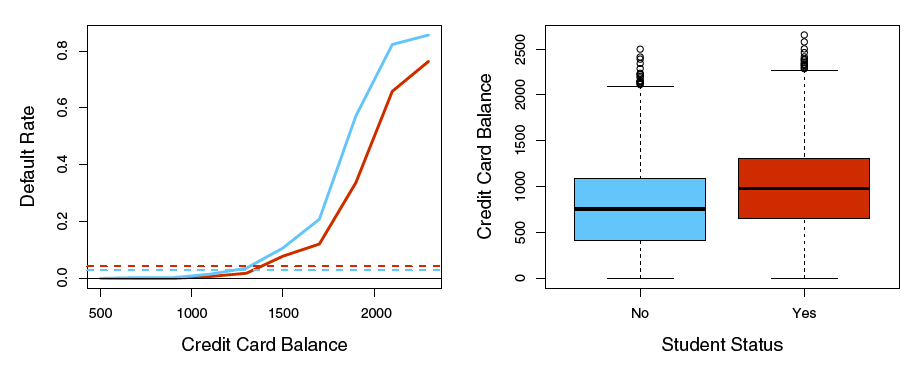
\includegraphics[width=0.8\textwidth]{images/islr/fig_4_3.png}
	\caption{A la izquierda, vemos que las tasas de impago para \textcolor{BrickRed}{estudiantes} y \textcolor{Cerulean}{no estudiantes}. La l\'inea s\'olida representa esta tasa en funci\'on del \vari{balance}, mientras que las l\'ineas horizontales punteadas son las tasas de impago generales. A la derecha, tenemos diagramas de caja para \textcolor{BrickRed}{estudiantes} y \textcolor{Cerulean}{no estudiantes}. Vemos que los estudiantes tienden a tener un \vari{balance} en la tarjeta de cr\'edito m\'as alto que los no estudiantes, pero para un \vari{balance} fijo, los estudiantes incurren menos en impago.}
	\label{fig:islr_4-3}
\end{figure}
\end{frame}

\begin{frame}\frametitle{Haciendo predicciones (3)}
\begin{itemize}
	\item ?`Cu\'al es la probabilidad de que una persona incurra en un \vari{impago} si es \vari{estudiante}, su \vari{balance} sea de $\$1,500$ y su \vari{salario} sea de $\$40,000$?
	\item Ingresamos los coeficientes encontrados:
	\begin{align*}
	\hat{p}(X)&=\frac{1}{1+\rm{e}^{10.869-0.005737\times 1500-0.000003\times40000+0.6468\times 1}}\\
	&= 0.0579=5.79\%
	\end{align*}
	\item ?`Cu\'al es la probabilidad de que una persona incurra en un \vari{impago} si no es \vari{estudiante}, su \vari{balance} sea de $\$1,500$ y su \vari{salario} sea de $\$40,000$?
	\item Ingresamos los coeficientes encontrados:
	\begin{align*}
	\hat{p}(X)&=\frac{1}{1+\rm{e}^{10.869-0.005737\times 1500-0.000003\times40000+0.6468\times 0}}\\
	&= 0.1049=10.49\%
	\end{align*}
\end{itemize}
\end{frame}

\begin{frame}\frametitle{Regresi\'on Log\'istica Multinomial (1)}
\begin{itemize}
	\item ?`Qu\'e pasa ahora si hay m\'as de dos clases, i.e., si $\mathcal{G}=\{1, \dotsc, K \}$?
	\item Se utiliza la \defi{regresi\'on log\'istica multinomial}.
	\item Decimos entonces que, para $k=1, \dotsc, K-1$:
	\[ \mathbb{P}[G=k|X=x] = \frac{\exp{(\beta_{k 0}+\beta_{k}^\top x)}}{1+\sum_{l=1}^{K-1}\exp{(\beta_{l 0}+\beta_{l}^\top x)}}\]
	y para $k=K$:
	\[ \mathbb{P}[G=K|X=x] = \frac{1}{1+\sum_{l=1}^{K-1}\exp{(\beta_{l 0}+\beta_{l}^\top x)}}\]
	
	
\end{itemize}
\end{frame}

\begin{frame}\frametitle{Regresi\'on Log\'istica Multinomial (2)}
\begin{itemize}
	\item N\'otese que esto induce fronteras de decisi\'on lineales: 
	\[ \{ x: \mathbb{P}[G=k|X=x] = \mathbb{P}[G=l|X=x] \}\]
	ser\'a equivalente a
	\[ \{ x: (\beta_{k0} - \beta_{l0})+(\beta_k - \beta_l)^\top x=0 \}\]
	
	\item Sin embargo, la regresi\'in log\'istica multinomial no es tan usada en la pr\'actica: es m\'as utilizado el \defi{an\'alisis discriminante}.
\end{itemize}
\end{frame}

\begin{frame}\frametitle{An\'alisis discriminante lineal (LDA)}
\begin{itemize}
	\item En regresi\'on log\'istica, modelamos directamente a $\mathbb{P}[G=k|X=x]$, i.e., modelamos a la distribuci\'on condicional de la respuesta $G$ dados los predictores $X$.
	\item Veremos otra alternativa: modelar a la distribuci\'on de los predictores $X$ para cada una de las clases de respuesta $G$ y luego usar el teorema de Bayes para encontrar a $\mathbb{P}[G=k|X=x]$.
	\item Si usamos a la distribuci\'on normal para cada clase, \'esto nos llevar\'a al an\'alisis discriminante lineal o cuadr\'atico.
	\item Se pueden utilizar otras distribuciones, pero nos enfocaremos en las normales.
\end{itemize}
\end{frame}

\begin{frame}\frametitle{?`Por qu\'e necesitamos otro modelo?}
\begin{itemize}
	\item Cuando las clases est\'an claramente separadas, las estimaciones de los par\'ametros dados por regresi\'on log\'istica son inestables (LDA no sufre de esto).
	\item Si $n$ es peque\~no y la distribuci\'on de las clases $X$ es aproximadamente normal, el modelo discriminante lineal es m\'as estable que el de regresi\'on log\'istica.
	\item LDA es m\'as popular que el model log\'istico cuando $|\mathcal{G}|>2$.
\end{itemize}
\end{frame}

\begin{frame}\frametitle{Usando el Teorema de Bayes para clasificaci\'on (1)}
\begin{itemize}
	\item Suponga que queremos clasificar una observaci\'on en una de las $K$ clases ($K\geq2$).
	\item Sea $\pi_k$ la \defi{probabilidad a priori} de que una observaci\'on escogida aleatoriamente pertenezca a la clase $k$.
	\item Representamos a la \defi{funci\'on de densidad de probabilidad} de que la observaci\'on $X$ pertenezca a la clase $k$ como
	\[ f_{k}(X)\equiv\mathbb{P}[X=x|G=k] \]
	\begin{itemize}
		\item $f_k(x)$ es relativamente grande si hay una alta probabilidad de que una observaci\'on en la clase $k$ tenga $X\approx x$.
	\end{itemize}
\end{itemize}
\end{frame}

\begin{frame}\frametitle{Usando el Teorema de Bayes para clasificaci\'on (2)}
\begin{itemize}
	\item Por lo tanto, el \textbf{teorema de Bayes} dice que:
	\begin{equation}
	\begin{aligned}\label{eq:islr_4-10}
	\mathbb{P}[G=k|X=x]&=\frac{\mathbb{P}[G=k]\cdot\mathbb{P}[X=x|G=k]}{\mathbb{P}[X=x]}\\
	&=\frac{\pi_k f_k(x)}{\sum_{j=1}^{K}\pi_j f_{j}(x)}=p_k(x)
	\end{aligned}
	\end{equation}
	\item Por lo tanto, de env\'es de calcular directamente a $p_k(x)$, utilizamos a las estimaciones de $\pi_k$ y $f_k(x)$ en la Ecuaci\'on \ref{eq:islr_4-10}.
	\item Nos referimos a $p_k(x)$ como la \defi{probabilidad a posteriori}.
\end{itemize}
\end{frame}

\begin{frame}\frametitle{Usando el Teorema de Bayes para clasificaci\'on (3)}
\begin{itemize}
	\item Podemos estimar a $\pi_k$ f\'acilmente: calculamos la fracci\'on de los datos de entrenamiento que pertenezcan a la clase $k$.
	\begin{itemize}
		\item Se debe de cumplir que	 $\sum_{k=1}^{K}\pi_k = 1$.
	\end{itemize}
	\item Estimar a $f_k(x)$ es m\'as complicado.
	\item Si logramos encontrar una manera de estimar a $f_k(x)$, podemos desarrollar a un clasificador que aproxime al clasificador de Bayes.
\end{itemize}
\end{frame}

\begin{frame}\frametitle{An\'alisis Discriminante Lineal para $p=1$ (1)}
\begin{itemize}
	\item Asumimos la forma de $f_k(x)$ como una funci\'on de densidad de una \defi{distribuci\'on normal} o \defi{Gaussiana}:
	\begin{equation}\label{eq:islr_4-11}
	f_k(x) = \frac{1}{\sqrt{2\pi}\sigma_{k}}\exp{\left( -\frac{1}{2\sigma_{k}^{2}}(x-\mu_k)^2 \right)}
	\end{equation}
	donde $\mu_k$ y $\sigma_k^2$ son los par\'ametros de media y varianza para la clase $k$.
	\item Asumamos, por ahora, que $\sigma_1^2=\dotsb=\sigma_K^2=\sigma^2$.
	\item Reemplazando a la Ecuaci\'on \ref{eq:islr_4-11} en la Ecuaci\'on \ref{eq:islr_4-10}, llegamos a:
	\begin{equation}\label{eq:islr_4-12}
	p_k(x)=\frac{\pi_k \frac{1}{\sqrt{2\pi}\sigma}\exp{\left( -\frac{1}{2\sigma^{2}}(x-\mu_k)^2 \right)}}{\sum_{j=1}^{K}\pi_j \frac{1}{\sqrt{2\pi}\sigma}\exp{\left( -\frac{1}{2\sigma^{2}}(x-\mu_j)^2 \right)}}
	\end{equation}
\end{itemize}
\end{frame}

\begin{frame}\frametitle{An\'alisis Discriminante Lineal para $p=1$ (2)}
\begin{itemize}
	\item Vemos lo siguiente:
	\begin{equation*}
	\begin{aligned}
	\log{\left(\frac{p_k(x)}{p_l(x)}\right)}&= \log{\left( \frac{\pi_k \exp{\left( -\frac{1}{2\sigma^{2}}(x-\mu_k)^2 \right)}}{\pi_l \exp{\left( -\frac{1}{2\sigma^{2}}(x-\mu_l)^2 \right)}} \right)}\\
	&= \log{\left( \frac{\pi_k}{\pi_l} \right)} - \frac{1}{2\sigma^{2}}(x-\mu_k)^2 + \frac{1}{2\sigma^{2}}(x-\mu_l)^2\\
	&= \log{\left( \frac{\pi_k}{\pi_l} \right)} - \frac{x^2}{2\sigma^2}+\frac{x \mu_k}{\sigma^2} -\frac{\mu_k^2}{2\sigma^2}+ \frac{x^2}{2\sigma^2} -\frac{x \mu_l}{\sigma^2} +\frac{\mu_l^2}{2\sigma^2}\\
	&= \log{\left( \frac{\pi_k}{\pi_l} \right)} + x \cdot\frac{\mu_k - \mu_l}{\sigma^2} - \frac{\mu_k^2-\mu_l^2}{2\sigma^2}
	\end{aligned}
	\end{equation*}
	\begin{itemize}
		\item !`Una funci\'on lineal!
	\end{itemize}
\end{itemize}
\end{frame}

\begin{frame}\frametitle{An\'alisis Discriminante Lineal para $p=1$ (3)}
\begin{itemize}
	\item Definimos a nuestra \defi{funci\'on discriminante lineal} como:
	\begin{equation}\label{eq:islr_4-13}
	\delta_k(x) = x\cdot \frac{\mu_k}{\sigma^2}-\frac{\mu_k^2}{2\sigma^2}+\log{\pi_k}
	\end{equation}
	\item Vemos que nuestra regla de decisi\'on se puede escribir de manera equivalente como:
	\[ G(x) = \argmax_k \delta_k(x) \]
	\item N\'otese, entonces, que $\log{\left(\frac{p_k(x)}{p_l(x)}\right)} = \delta_k(x)-\delta_l(x)$
	\item Si $K=2$ y $\pi_1=\pi_2$, entonces la frontera de decisi\'on de Bayes corresponde al punto donde
	
	\[ x=\frac{\mu_1^2-\mu_2^2}{2(\mu_1-\mu_2)}=\frac{\mu_1+\mu_2}{2} \]
\end{itemize}
\end{frame}

\begin{frame}\frametitle{Clasificamos a la densidad m\'as alta}
\begin{figure}
	\centering
	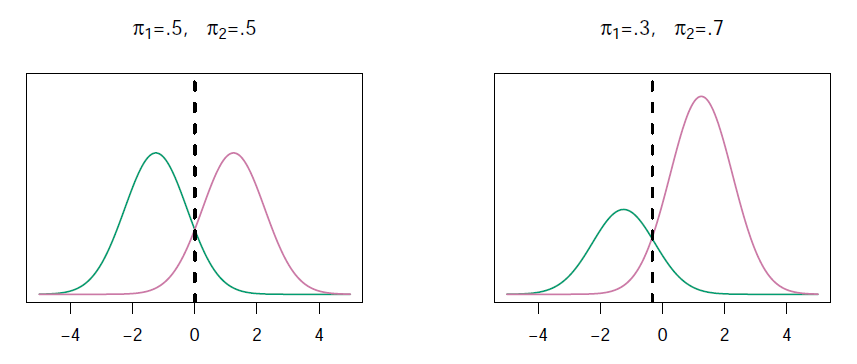
\includegraphics[width=0.8\textwidth]{images/islr_lectures/densidad_alta.png}
	\caption{Clasificamos a un dato de acorde con cu\'al $\pi_k f_k(x)$ es m\'as alto o, de manera equivalente, cu\'al discriminante lineal $\delta_k(x)$ es m\'as alto. A la derecha, favorecemos a la clase \textcolor{Orchid}{morada}, por lo que la frontera de decisi\'on se ha corrido a la izquierda. En ambos casos, tendremos que $\mu_1=-1.25$, $\mu_2=1.25$ y $\sigma_1=\sigma_2=1$.}
	\label{fig:islr_lectures-densidad_alta}
\end{figure}
\end{frame}

\begin{frame}\frametitle{An\'alisis Discriminante Lineal para $p=1$ (4)}
\begin{itemize}
	\item En la vida real, aunque estemos seguros de nuestra suposici\'on de que $X$ tiene una distribuci\'on normal ($X\sim \mathcal{N}(\mu, \sigma^2)$), a\'un tendremos que estimar a los par\'ametros $\mu_1, \dotsc, \mu_K$, $\pi_1, \dotsc, \pi_K$ y a $\sigma^2$. 
	\item El m\'etodo de \defi{An\'alisis Discriminante Lineal (LDA)} aproxima al clasificador de Bayes al ingresar, en la Ecuaci\'on \ref{eq:islr_4-13}, estimaciones de dichos par\'ametros.
	\item Utilizaremos las siguientes:
	\begin{equation}\label{eq:islr_4-15-a}
	\hat \mu_k = \frac{1}{n_k} \sum_{i:g_i=k}x_i
	\end{equation}
	
	\begin{equation}\label{eq:islr_4-15}
	\hat \sigma^2 = \frac{1}{n - K} \sum_{k=1}^{K}\sum_{i:g_i=k}(x_i-\hat \mu_k)^2
	\end{equation}
	donde $n=|\mathcal{T}_{\text{Tr}}|$ (el n\'umero total de observaciones de entrenamiento) y $n_k$ es el n\'umero de observaciones de entrenamiento en la clase $k$.
\end{itemize}
\end{frame}

\begin{frame}\frametitle{An\'alisis Discriminante Lineal para $p=1$ (5)}
\begin{itemize}
	\item A veces se tiene conocimiento de las probabilidades a priori $\pi_1, \dotsc, \pi_K$, por lo que podemos utilizarlas directamente.
	\item De lo contrario, usamos a las proporciones en los datos de entrenamiento por clase:
	\begin{equation}\label{eq:islr_4-16}
	\hat \pi_k = n_k/n
	\end{equation}
	\item Por lo tanto, el \defi{clasificador LDA} asigna a una observaci\'on $X=x$ la clase para la cual la funci\'on discriminante
	\begin{equation}\label{eq:islr_4-17}
	\hat \delta_k(x) = x\cdot \frac{\hat\mu_k}{\hat\sigma^2}-\frac{\hat\mu_k^2}{2\hat\sigma^2}+\log{\hat\pi_k}
	\end{equation}
	es mayor, i.e., $G = \argmax_k \hat \delta_k(x)$.
\end{itemize}
\end{frame}

\begin{frame}\frametitle{Frontera de decisi\'on del LDA}
\begin{figure}
	\centering
	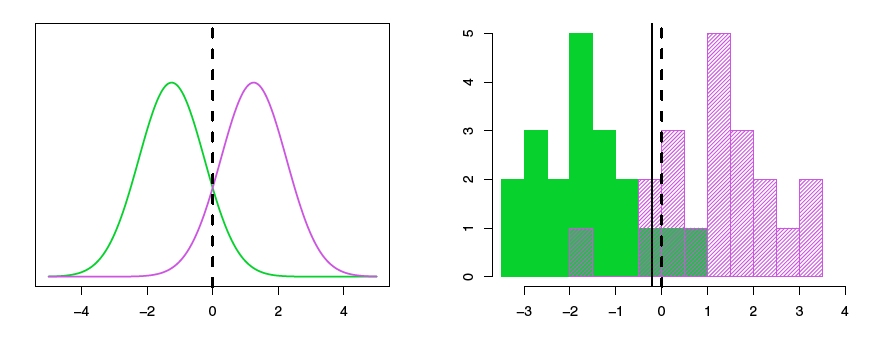
\includegraphics[width=0.8\textwidth]{images/islr/fig_4_4.png}
	\caption{En ambas gr\'aficas, la l\'inea vertical punteada nos muestra la frontera de decisi\'on de Bayes, $x=(\mu_1 + \mu_2)/2$, para dos funciones de densidad normales, con $\mu_1=-1.25$, $\mu_2=1.25$, $\sigma_1^2=\sigma_2^2=1$ y $\pi_1=\pi_2=0.5$. A la derecha, hemos tomado 20 observaciones de cada clase ($n_1=n_2=20$) y mostramos el histograma. La l\'inea negra s\'olida representa la frontera de decisi\'on del LDA que ha sido estimado de los datos, i.e., $x=(\hat \mu_1 + \hat \mu_2)/2$. El error de Bayes es de $10.6\%$ y el error del LDA es de $11.1\%$.}
	\label{fig:islr_4-4}
\end{figure}
\end{frame}

\begin{frame}\frametitle{An\'alisis Discriminante Lineal para $p>1$ (1)}
\begin{itemize}
	\item Tendremos ahora que $X=(X_1, \dotsc, X_p)$ tiene una \defi{distribuci\'on normal (Gausiana) multivariante}: $X\sim\mathcal{N}(\bm{\mu},\bm{\Sigma})$, donde $\bm{\mu}=(\mu_1,\dotsc, \mu_p)$ y $\bm{\Sigma}$, la matriz $p\times p$ de covarianza de $X$: \[\bm \Sigma=\text{Cov}(X)=\mathbb{E}\left [X X^\top\right ]-\bm \mu \bm \mu^\top\]
	\item En otras palabras, asumimos que cada predictor sigue una distribuci\'on normal unidimensional, con alguna correlaci\'on entre cada par de predictores $X_i$ y $X_j$ dada por $\bm\Sigma_{ij}$.
	\item La funci\'on de densidad est\'a dada por:
	\begin{equation}\label{eq:islr_4-18}
	f(x) = \frac{1}{(2\pi)^{p/2}|\bm\Sigma|^{1/2}}\exp{\left( -\frac{1}{2} (x-\bm \mu)^{\top}\bm \Sigma^{-1}(x-\bm \mu) \right)}
	\end{equation}
\end{itemize}
\end{frame}

\begin{frame}\frametitle{Distribuci\'on normal multivariante con $p=2$}
\begin{figure}
	\centering
	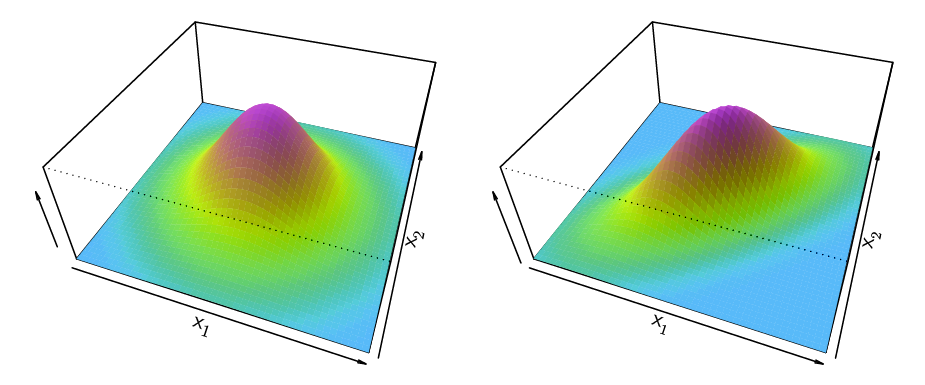
\includegraphics[width=0.8\textwidth]{images/islr/fig_4_5.png}
	\caption{Dos funciones de densidad normal multivariantes, con $p=2$. A la izquierda, los predictores $X_1$ y $X_2$ tienen misma varianza, $\mathbb{V}[X_1]=\mathbb{V}[X_2]$ y no est\'an correlacionados, por lo que $\text{Cor}(X_1, X_2)=0$. A la derecha, los predictores tienen una correlaci\'on de $0.7$. La base de la campana ya no es circular, sino el\'iptica.}
	\label{fig:islr_4-5}
\end{figure}
\end{frame}

\begin{frame}\frametitle{An\'alisis Discriminante Lineal para $p>1$ (2)}
\begin{itemize}
	\item En otras palabras, las observaciones en la clase $k$ se extraen de una distribuci\'on normal multivariante $\mathcal{N}(\mu_k,\bm \Sigma)$.
	\item El clasificador de Bayes asigna una observaci\'on $X=x$ a la clase para la cual la funci\'on discriminante
	\begin{equation}\label{eq:islr_4-19}
	\delta_k(x) = x^\top \bm \Sigma^{-1}\mu_k-  \frac{1}{2}\mu_k^{\top}\bm\Sigma^{-1}\mu_k+\log{\pi_k}
	\end{equation}
	es mayor, i.e., $G = \argmax_k \delta_k(x)$.
	\item La versi\'on matricial de la Ecuaci\'on \ref{eq:islr_4-13}.
	\item Sigue siendo una funci\'on lineal.
	\item Necesitaremos aproximaciones a los par\'ametros, por lo que utilizamos las versiones matriciales de las Ecuaciones \ref{eq:islr_4-15-a}, \ref{eq:islr_4-15} y \ref{eq:islr_4-16}.
\end{itemize}
\end{frame}

\begin{frame}\frametitle{Dos predictores $p=2$ y $K=3$ clases}
\begin{figure}
	\centering
	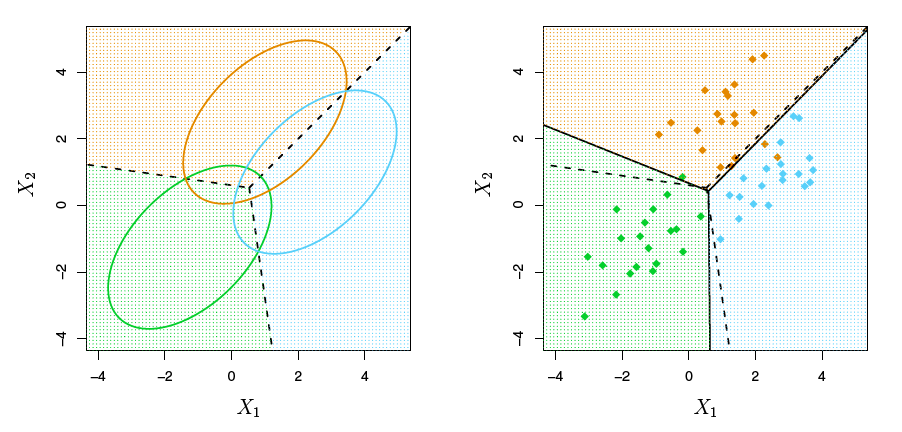
\includegraphics[width=0.7\textwidth]{images/islr/fig_4_6.png}
	\caption{Se muestran tres clases Gausianas de igual tama\~no, con un vector de la media espec\'ifico por clase, as\'i como una matriz de covarianza com\'un para las tres clases. Las elipses representan las regiones que contienen el $95\%$ de los datos de cada una de las clases. Las l\'ineas punteadas son las fronteras de decisi\'on de Bayes, i.e., donde $\delta_k(x)=\delta_l(x)$. Tendremos que $\pi_1=\pi_2=\pi_3=1/3$. A la derecha se han generado 20 observaciones por clase y se muestran las fronteras de decisi\'on del LDA con una l\'inea negra s\'olida. El error de prueba de Bayes es de $0.0746$ y el del LDA es de $0.0770$.}
	\label{fig:islr_4-6}
\end{figure}
\end{frame}

\begin{frame}\frametitle{Llev\'andolo a probabilidades}
\begin{itemize}
	\item Otra manera de facilitar la interpretaci\'on de las funciones discriminantes $\hat \delta_k (x)$ es transformando los resultados a probabilidades.
	\item Lo logramos mediante la \defi{funci\'on Softmax}:
	\begin{equation}\label{eq:softmax}
	\hat{\mathbb{P}}[G=k|X=x]=\frac{\exp{\hat \delta_k(x)}}{\sum_{l=1}^{K}\exp{\hat \delta_l(x)}}
	\end{equation}
	\item As\'i, normalizamos a los valores obtenidos para que est\'en en el rango $[0,1]$ y que su suma sea igual a $1$.
	\item Cuando $p=2$, lo usual es asignar a una clase si la probabilidad es mayor a $0.5$, i.e., si $\hat{\mathbb{P}}[G=k|X=x]\geq 0.5$.
	\item Se pueden usar otros l\'imites, dependiendo de la aplicaci\'on y qu\'e tan conservador es uno.
\end{itemize}
\end{frame}


\begin{frame}[fragile]\frametitle{C\'odigo LDA, $p=2$ y $K=2$}
\begin{semiverbatim}
	\footnotesize{\textcolor{deepblue}{import} pandas \textcolor{deepblue}{as} pd
		\textcolor{deepblue}{from} sklearn.discriminant\_analysis \textcolor{deepblue}{import} LinearDiscriminantAnalysis
		
		df = \href{https://pandas.pydata.org/pandas-docs/stable/reference/api/pandas.read_excel.html}{pd.read\_excel}(\href{https://goo.gl/qSE6q8}{"https://goo.gl/qSE6q8"})
		
		# .factorize() nos regresa dos objetos: un array con etiquetas
		# y uno con valores unicos. Solo nos interesa el primero:
		df["default2"] = df.default.\href{https://pandas.pydata.org/pandas-docs/version/0.23.4/generated/pandas.factorize.html}{factorize()}[0]
		df["student2"] = df.student.\href{https://pandas.pydata.org/pandas-docs/version/0.23.4/generated/pandas.factorize.html}{factorize()}[0]
		
		y = df.default2.values
		X = df[["balance", "student2"]].values
		
		lda = \href{https://scikit-learn.org/stable/modules/generated/sklearn.discriminant_analysis.LinearDiscriminantAnalysis.html#sklearn.discriminant_analysis.LinearDiscriminantAnalysis}{LinearDiscriminantAnalysis}().fit(X, y)
		y\_pred = lda.predict(X)
		
		>>> print("Error: \{:.2f\}".format(100*(1 - sum(y == y\_pred)/len(y))), "\%")
		>>> print("Error: \{:.2f\}".format(100*(1 - lda.score(X, y))), "\%")\footnote{?`Es un buen modelo?}
	}
\end{semiverbatim}
\end{frame}

\begin{frame}\frametitle{An\'alisis del LDA}
\begin{itemize}
	\item El error del LDA es de $2.75\%$, pero debemos de tener en mente dos cosas:
	\begin{itemize}
		\item Estamos hablando de error de entrenamiento, por lo que mientras m\'as alta es la raz\'on $p/n$, es m\'as probable que estemos \textit{sobreajustando}. No es el caso aqu\'i, ya que $p=2$ y $n=10,000$.
		\item Ya que s\'olo el $3.33\%$ de los individuos en los datos incurrieron en un impago un \defi{clasificador nulo} que clasifica a todos como \vari{No} har\'ia un trabajo comparable con nuestro clasificador LDA.
		\item Podemos conseguir lo \'ultimo mediante \texttt{100*sum(y)/len(y)}.
	\end{itemize}
	\item Podemos realizar dos tipos de error: asignarle incorrectamente a un individuo que incurre en un impago la categor\'ia \vari{No} (\defi{Error tipo I}) o asignarle incorrectamente a un individuo que no incurre en un impago la categor\'ia \vari{Si} (\defi{Error tipo II}).
\end{itemize}
\end{frame}

\begin{frame}\frametitle{M\'etricas a seguir (1)}
\begin{itemize}
	\item Generalmente deseamos saber qu\'e tipo de error estamos cometiendo.
	\item Utilizamos una \defi{matriz de confusi\'on} para desplegar esta informaci\'on.
	\item Para una respuesta binaria, tendremos cuatro elementos en nuestra matriz de confusi\'on:
	\begin{itemize}
		\item \defi{Verdadero negativo (TN)} cuando $\hat G = \vari{No}$ y $G=\vari{No}$.
		\item \defi{Verdadero positivo (TP)} cuando $\hat G = \vari{Si}$ y $G=\vari{Si}$ (\defi{potencia}).
		\item \defi{Falso negativo (FN)} cuando $\hat G = \vari{No}$ y $G=\vari{Si}$ (error tipo II).
		\item \defi{Falso positivo (FP)} cuando $\hat G = \vari{Si}$ y $G=\vari{No}$ (error tipo I).
	\end{itemize}
\end{itemize}
\end{frame}

\begin{frame}\frametitle{M\'etricas a seguir (2)}
\begin{itemize}
	\item Con \'estos, podemos definir a otras tres m\'etricas:
	\begin{itemize}
		\item \defi{Sensibilidad o exhaustividad (True Positive Rate, TPR)}: el porcentaje de individuos que realmente incurren en un impago que son correctamente identificados:
		\[ \text{Sensibilidad} = \frac{\text{TP}}{\text{TP}+ \text{FN}} = \text{TPR}=\text{recall}\]
		\item \defi{Especificidad (True Negative Rate, TNR)}: el porcentaje de individuos que no incurren en un impago que son correctamente identificados:
		\[ \text{Especificidad} = \frac{\text{TN}}{\text{TN}+ \text{FP}} = \text{TNR}\]
		\item \defi{Precisi\'on}: el porcentaje de individuos que incurren en un impago que son identificados:
		\[ \text{Precisi\'on} = \frac{\text{TP}}{\text{TP}+ \text{FP}}\]
		
	\end{itemize}

\end{itemize}
\end{frame}



\begin{frame}[fragile]\frametitle{Matriz de confusi\'on}
\begin{semiverbatim}
	\textcolor{deepblue}{from} sklearn.metrics \textcolor{deepblue}{import} \href{https://scikit-learn.org/stable/modules/generated/sklearn.metrics.confusion_matrix.html}{confusion\_matrix}
y\_actual = pd.Series(y, name="Actual")
y\_predicted = pd.Series(y\_pred, name="Predicho")

y\_actual = y\_actual.\href{https://pandas.pydata.org/pandas-docs/stable/reference/api/pandas.DataFrame.replace.html}{replace}([0, 1], ["No", "Si"])
y\_predicho = y\_predicho.\href{https://pandas.pydata.org/pandas-docs/stable/reference/api/pandas.DataFrame.replace.html}{replace}([0, 1], ["No", "Si"])

>>> pd.crosstab(y\_actual, y\_predicho, margins=True)

>>> print(confusion\_matrix(y\_actual, y\_pred))

tn, fp, fn, tp = confusion\_matrix(y, y\_pred).ravel()

\end{semiverbatim}
\end{frame}

\begin{frame}\frametitle{M\'etricas a seguir (3)}
\begin{itemize}
	\item Definimos al \defi{error total cometido} como $(\text{FP} + \text{FN} )/ n$
	\item La \defi{tasa de falsos negativos (FNR)} es la proporci\'on de individuos que incurrieron en un impago que fueron clasificados como \vari{No}:
	\[ \text{FNR} = \frac{\text{FN}}{\text{FN}+ \text{TP}}\]
	
	\item La \defi{tasa de falsos positivos (FPR)} es la proporci\'on de individuos que no incurrieron en un impago que fueron clasificados como \vari{Si}:
	\[ \text{FPR} = \frac{\text{FP}}{\text{FP}+ \text{TN}}\]
	\item El \defi{valor F balanceado (F1)} es la media harm\'onica entre precisi\'on y exhaustividad:
	
	\[ F_1 = \frac{2}{\text{precisi\'on}^{-1}+\text{exhaustividad}^{-1}}  =\frac{2 \text{TP}}{2\text{TP}+\text{FP} + \text{FN}} \]
\end{itemize}
\end{frame}

\begin{frame}\frametitle{Modificando al umbral}
\begin{itemize}
	\item Una compa\~n\'ia de tarjetas de cr\'edito puede estar m\'as interesada en evitar el Error tipo II que el Error tipo I. 
	\item En otras palabras, le es preferible no dar una tarjeta de cr\'edito a un individuo que no va a incurrir en un impago que darsela a uno que s\'i va a incurrir en un impago.
	\item Podemos, entonces modificar al umbral de decisi\'on para clasificar a los individuos/clientes como aquellos que \vari{Si} incurrir\'an en un impago a uno m\'as bajo, i.e., pasar de
	
	\begin{equation}\label{eq:islr_4-21} \hat{\mathbb{P}}[\vari{impago}=\vari{Si}|X=x] >0.5 
	\end{equation}
	a
	\begin{equation}\label{eq:islr_4-22} 
	\hat{\mathbb{P}}[\vari{impago}=\vari{Si}|X=x] >0.2 
	\end{equation}
	\item El Error tipo II baja de $252/333=75.7\%$ a $138/333=41.4\%$, mientras que el Error tipo I sube de $23/9667=0.238\%$ a $235/9667=2.43\%$. A la compa\~n\'ia le puede parecer aceptable.
\end{itemize}
\end{frame}

\begin{frame}\frametitle{C\'odigo para M\'etricas y Umbral}

\begin{center}
	Link al c\'odigo:
	\href{https://goo.gl/vPNmpB}{https://goo.gl/vPNmpB}
\end{center}
\begin{itemize}
	\item Vemos que podemos seguir modificando el umbral y ver el intercambio que sucede entre las m\'etricas.
	\item Seleccionar el umbral correcto depende del \textit{conocimiento del campo} (e.g., los costos incurridos al cometer los tipos de errores).
	\item El error total baja pero la FNR sube.
\end{itemize}
\end{frame}

\begin{frame}\frametitle{Curva ROC}
\begin{itemize}
	\item Una \defi{curva ROC} muestra el desempe\~no de un clasificador con todos los umbrales posibles al comparar la tasa de falsos positivos versus la tasa de verdaderos positivos.
	\item Podemos resumir al clasificador por el \defi{\'area bajo la curva (AUC)}.
	\item Una curva ROC ideal se aferrar\'a a la esquina superior izquierda, por lo que $\text{AUC}=1$.
	\item Un clasificador que no es mejor que una decisi\'on aleatoria tendr\'a $\text{AUC}=0.5$, o un ROC que es una l\'linea a $45\textdegree$.
\end{itemize}
\end{frame}

\begin{frame}\frametitle{Curva ROC para los datos de \vari{Default}}
\begin{figure}
	\centering
	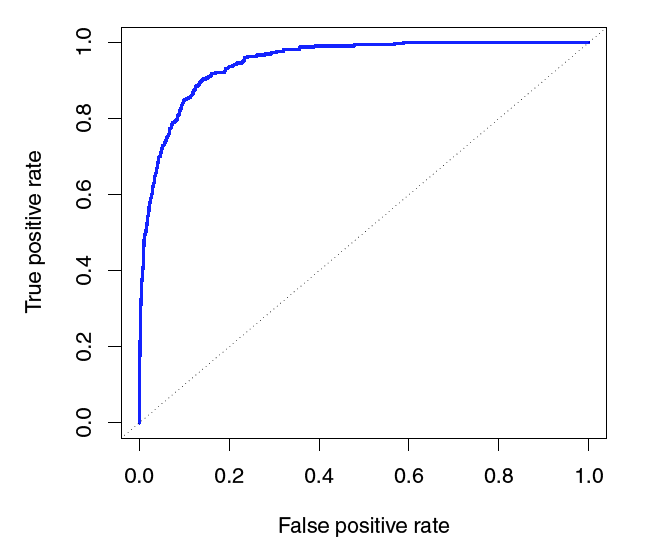
\includegraphics[width=0.5\textwidth]{images/islr/fig_4_8.png}
	\caption{La curva ROC para el clasificador LDA en los datos de \vari{Default}. Conforme modifiquemos el umbral, cambiar\'an tanto el FPR como el TPR. La l\'inea punteada es el clasificador que no es mejor que una decisi\'on aleatoria. Por lo tanto, deseamos que nuestro clasificador est\'e siempre por arriba de dicha l\'inea.}
	\label{fig:islr_4-8}
\end{figure}
\end{frame}

\begin{frame}\frametitle{An\'alisis Discriminante Cuadr\'atico (QDA)}
\begin{itemize}
	\item El \defi{an\'alisis discriminante cuadr\'atico (QDA)} tiene las mismas suposiciones que el LDA, excepto que ahora asumimos que cada clase tiene su propia matriz de covarianza $\bm \Sigma_k$.
	\item Por lo tanto, dichos t\'erminos no van a desaparecer y definimos a la \defi{funci\'on discriminante cuadr\'atica}:
	\begin{equation}\label{eq:islr_4-23}
	\begin{aligned}
	\delta_k(x) &= -\frac{1}{2}(x-\bm{\mu}_{k})^{\top} \bm{\Sigma}_k^{-1}(x-\bm{\mu}_k) - \frac{1}{2}\log{|\bm \Sigma_k|} + \log{\pi_k}\\
	&= -\frac{1}{2} x^{\top}\bm{\Sigma}_k^{-1} x + x^{\top}\bm{\Sigma}_k^{-1} \bm \mu_k - \frac{1}{2}\bm \mu_k^{\top}\bm{\Sigma}_k^{-1}\bm \mu_k- \frac{1}{2}\log{|\bm \Sigma_k|} + \log{\pi_k}
	\end{aligned}
	\end{equation}
	\item La frontera de decisi\'on $\{x:\delta_k(x) = \delta_l(x) \}$ ser\'an ecuaciones cuadr\'aticas.
	\item Nuestra decisi\'on ser\'a nuevamente: $G=\argmax_k \delta_k(x)$. De manera equivalente, podemos calcular las probabilidades utilizando a la Ecuaci\'on \ref{eq:softmax} (funci\'on Softmax).
\end{itemize}
\end{frame}

\begin{frame}\frametitle{LDA vs. QDA para dos casos}
\begin{figure}
	\centering
	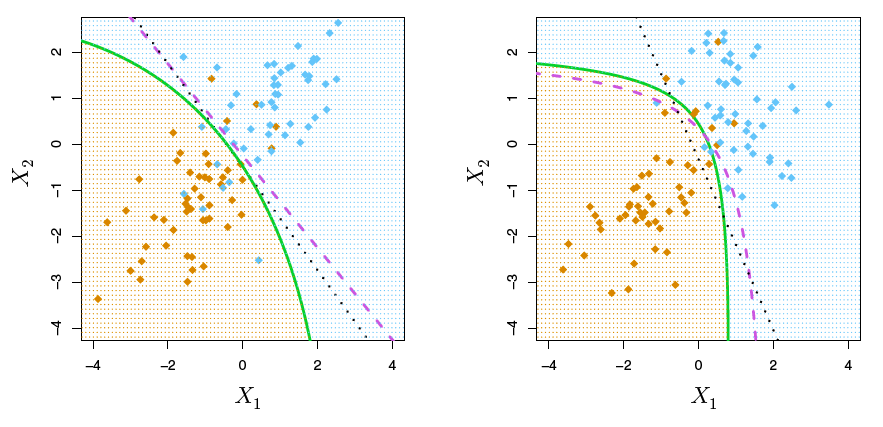
\includegraphics[width=0.75\textwidth]{images/islr/fig_4_9.png}
	\caption{Presentamos a la frontera de decisi\'on del LDA es la l\'inea negra punteada; la del QDA es la l\'inea \textcolor{green}{verde} y la de Bayes es la l\'inea punteada \textcolor{Orchid}{morada}. A la derecha, tendremos datos generados con $\bm \Sigma_1 = \bm \Sigma_2$ y podemos apreciar que la frontera de decisi\'on de Bayes es lineal, por lo que LDA la aproxima mejor. A la izquerda, tendremos que $\bm \Sigma_1 \neq \bm \Sigma_2$ y la frontera de decisi\'on de Bayes es no lineal, por lo que QDA la aproxima mejor.}
	\label{}
\end{figure}
\end{frame}

\begin{frame}\frametitle{LDA vs. QDA}
\begin{itemize}
	\item Cuando tenemos $p$ predictores, estimar la matriz de covarianza requiere de estimar a $p(p+1)/2$ par\'ametros.
	\item Por lo tanto, ya que QDA requiere de $K$ distintas covarianzas, se tendr\'an que estimar $K p(p+1)/2$ par\'ametros.
	\item En cambio, LDA es un modelo lineal, por lo que se requieren estimar a $K p$ par\'ametros.
	\item Por lo tanto, LDA es mucho menos flexible que QDA y tiene menor varianza, pero mayor sesgo. 
	\item LDA realiza un mejor trabajo que QDA si hay pocos datos de entrenamiento; se recomienda usar a QDA si el conjunto de entrenamiento es muy grande y la varianza del clasificador no es una preocupaci\'on.
\end{itemize}
\end{frame}

\begin{frame}\frametitle{KNN}
\begin{itemize}
	\item El \defi{clasificador de k vecinos cercanos (KNN)} no asume la distribuci\'on de los datos.
	\item Primero identifica a los $K$ puntos m\'as cercanos a una observaci\'on de prueba $x_0$, los cuales representamos por $\mathcal{N}_0$.
	\item Estimamos a la probabilidad condicional de que dicho punto pertenezca a la clase $j$ como:
	\begin{equation}\label{eq:islr_2-12}
	\mathbb{P}[G=j|X=x_0]=\frac{1}{K}\sum_{i \in\mathcal{N}_0}\mathbbm{1}_{g_i=j}(x_0)
	\end{equation}
	\item La elecci\'on de $K$ tiene efectos dram\'aticos en el clasificador obtenido.
\end{itemize}
\end{frame}

\begin{frame}\frametitle{Ilustraci\'on de KNN}
\begin{figure}
	\centering
	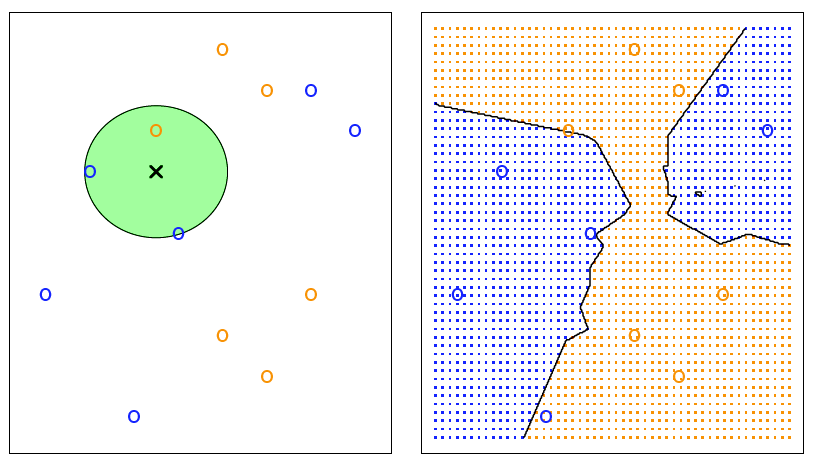
\includegraphics[width=0.8\textwidth]{images/islr/fig_2_14.png}
	\caption{Usando a $K=3$, el c\'irculo verde nos indica que, para clasificar a un punto que se localiza en la cruz, debemos de tomar en consideraci\'on a los dos puntos azules y al punto anaranjado. A la derecha mostramos las fronteras de decisi\'on generadas con los datos y n\'umero de vecinos cercanos.}
	\label{fig:islr_2-14}
\end{figure}
\end{frame}

\begin{frame}[fragile]\frametitle{C\'odigo KNN}
\begin{semiverbatim}
	\textcolor{deepblue}{from} sklearn.neighbors \textcolor{deepblue}{import} \href{https://scikit-learn.org/stable/modules/generated/sklearn.neighbors.KNeighborsClassifier.html}{KNeighborsClassifier}
	knn = KNeighborsClassifier(n\_neighbors=3)
	
	knn.fit(X, y)
	
	y\_predicho = knn.predict(X)
	
	>>> print(confusion\_matrix(y, y\_pred))
	
	tn, fp, fn, tp = confusion\_matrix(y, y\_pred).ravel()
	
\end{semiverbatim}
\end{frame}

\begin{frame}\frametitle{Variando a K en KNN}
\begin{figure}
	\centering
	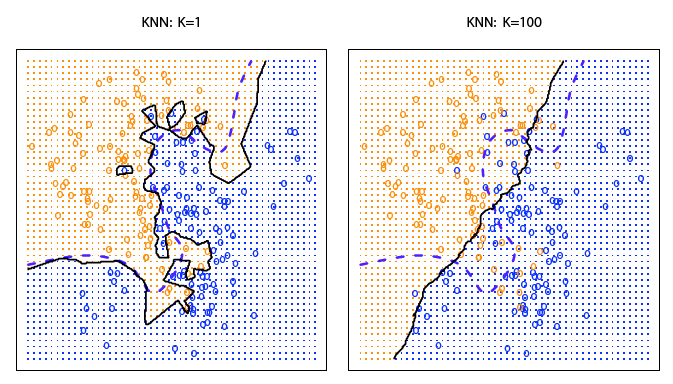
\includegraphics[width=0.8\textwidth]{images/islr/fig_2_16.png}
	\caption{A la izquierda, usamos $K=1$ vecinos cercanos, mientras que a la derecha usamos $K=100$ vecinos cercanos para datos generados. La frontera de decisi\'on de Bayes es la l\'inea punteada. N\'otese que, conforme aumentemos a $K$, la frontera de decisi\'on de KNN se vovler\'a cada vez m\'as lineal (menos flexible).}
	\label{fig:islr_2-16}
\end{figure}
\end{frame}

\begin{frame}\frametitle{\'Ultimas notas}
\begin{itemize}
	\item Existe otro tipo de funci\'on discriminante llamado \defi{Naive Bayes}.
	\item Es \'util cuando tenemos predictores cualitativos y cuantitativos, as\'i como cuando $p$ es muy grande.
	\item Tendremos que:
	\begin{equation*}
	\begin{aligned} \delta_k(x) &\propto \log{\left[ \pi_k \prod_{j=1}^{p}f_{kj}(x_j) \right]}\\
	&=-\frac{1}{2}\sum_{j=1}^{p}\left[\frac{(x_j-\mu_{kj})^2}{\sigma_{kj}^2} +\log{\sigma_{kj}^2}\right]+\log{\pi_k} 
	\end{aligned}
	\end{equation*}
	\item A pesar de sus suposiciones fuertes, usualmente produce buenos resultados.
\end{itemize}
\end{frame}

\end{document}